\section{Basic Statistical Descriptors of Data}

\begin{frame}{Basic Statistical Descriptions of Data}
	\textbf{Motivation}:
	\begin{itemize}
		\item To better understand the data: central tendency, variation and spread.
	\end{itemize}

	\textbf{Data dispersion characteristics}:
	\begin{itemize}
		\item Median, max, min, quantiles, outliers, variance etc.
	\end{itemize}

	\textbf{Numerical dimensions correspond to sorted intervals.}\\
	\begin{itemize}
		\item Data dispersion: analyzed with multiple granularities of precision.
		\item Boxplot or quantile analysis on sorted intervals
	\end{itemize}

	\textbf{Dispersion analysis on computed measures.}\\
	\begin{itemize}
		\item Folding measures into numerical dimensions.
		\item Boxplot or quantile analysis on the transformed cube.
	\end{itemize}
\end{frame}

\begin{frame}{Population vs. Sample}
	\begin{columns}[t]
		\begin{column}{0.5\columnwidth}
			\centering \textbf{Population}
			\begin{itemize}
				\item Collection of \textit{all} data objects of interest.\\ E.g. all
				      people currently living in Germany or all enrolled students at FAU.
				\item Population size often denoted by $N$.
				\item Hard to define and to observe.\\E.g. a survey requiring all enrolled
				      students is often not feasible as not all will participate.
			\end{itemize}
			\begin{alertblock}{Note}
				Unlikely that we have data of a whole population. Thus, we can assume we
				always have a sample.
			\end{alertblock}
		\end{column}
		\begin{column}{0.5\columnwidth}
			\centering \textbf{Sample}
			\begin{itemize}
				\item Randomly selected and representative subset of a population obtained
				      by a sampling method\footnote[frame]{Example include but not limited to
					      simple random sampling, stratified sampling.}.
				\item Sample size often denoted by $n$.
				\item Sample guards against (unconscious) investigator biases.
				\item Samples are faster and less costly to obtain.
				\item More control regarding (missing) values and outlier.
			\end{itemize}
		\end{column}
	\end{columns}
\end{frame}

\begin{frame}{Measuring the Central Tendency: Mean and Trimmed Mean}
	\begin{columns}
		\begin{column}{0.5\textwidth}
			\textbf{Arithmetic Mean}

			Simple and most commonly used measure of central tendency:

			\begin{equation*}
				\bar{x} = \frac{1}{n} \sum_{i=1}^{n} x_i.
			\end{equation*}

			\begin{itemize}
				\item Sensitive to extreme values (outliers).
			\end{itemize}
		\end{column}
		\begin{column}{0.5\textwidth}
			\textbf{Trimmed Mean}

			Simple and robust variation of the arithmetic mean:
			\begin{equation*}
				\bar{x} = \frac{x_{([n\alpha]+1)}+ \dots x_{(n-[n\alpha])}}{n-2[n\alpha]}
			\end{equation*}
			where $[n\alpha]$ denotes the greatest index less than or equal to $n\alpha$. In other words:

			\begin{itemize}
				\item Order data.
				\item Discard lowest $100\alpha\%$ and highest $100\alpha\%$.
				\item Compute arithmetic mean on remaining data.
			\end{itemize}


			Note: 50\% trimmed mean corresponds to median.
		\end{column}
	\end{columns}
\end{frame}

\begin{frame}{Measuring the Central Tendency: Median (I)}
	The \textbf{median} $\tilde{x}$ is the middle value of ordered observations where
	\begin{itemize}
		\item A minimum of 50\% of all values are lesser or equal $\tilde{x}$.
		\item A minimum of 50\% of all values are greater or equal $\tilde{x}$.
	\end{itemize}

	\begin{align*}
		\tilde{x} = %
		\begin{cases}
			x_{\frac{N}{2}}                               & \text{if $N$ mod $2 = 0$,}    \\
			\frac{x_{\frac{N-1}{2}}+x_{\frac{N+1}{2}}}{2} & \text{if $N$ mod $2 \neq 0$.}
		\end{cases}
	\end{align*}
	More robust compared to mean as extreme values does not have such drastic affects.
\end{frame}

\begin{frame}{Measuring the Central Tendency: Median (II)}
	\textbf{Median for interval grouped data} (An Example)
	\begin{table}
		\begin{tabularx}{\textwidth}{|c|c|p{4.5em}|X|X|X|}
			\hline
			\rowcolor{faugray!62}\textbf{Class $i$} & \textbf{Age $x_i$} ($x_i^l$ - $x_i^u$) & \textbf{Class Width $\Delta_i$} & \textbf{Absolute\newline Frequency $n_i$} & \textbf{Relative\newline Frequency $f_i$} & \textbf{Cumulative rel.\newline Frequency $F_i$} \\ \hline
			$1$                                     & $1-5$                                  & 4                               & $200$                                     & 0.06262                                   & 0.06262                                          \\
			$2$                                     & $6-15$                                 & 9                               & $450$                                     & 0.14089                                   & 0.20351                                          \\
			$3$                                     & $16-20$                                & 4                               & $300$                                     & 0.09393                                   & 0.29743                                          \\
			\rowcolor{fauyellow!62} $4$             & $21-50$                                & 29                              & $1500$                                    & 0.46963                                   & 0.76706                                          \\
			$5$                                     & $51-80$                                & 29                              & $700$                                     & 0.21916                                   & 0.98622                                          \\
			$6$                                     & $81-110$                               & 29                              & $44$                                      & 0.01378                                   & 1.00000                                          \\ \hline
			$\sum$                                  &                                        &                                 & 3194                                      & 1.00000                                   &                                                  \\ \hline
		\end{tabularx}
	\end{table}

	The median lies within the fourth group, i.e. in the age group from 21 to 50 years
\end{frame}

\begin{frame}{Measuring the Central Tendency: Median (III)}
	\textbf{Median for interval grouped data}

	For grouped data we typically have no information about the underlying
	distribution. However, we can assume that the data is equally
	distributed. In this case we can approximate the median with the following
	steps:
	\begin{itemize}
		\item Order data (in our example by age, not by frequencies!).
		\item Compute relative frequencies, that is: frequency divided by sum of all frequencies.
		\item Compute cumulative relative frequencies.
	\end{itemize}

	Determine median with these considerations:
	\begin{itemize}
		\item $F_i=0.5$: We have no clear median. Therefore: Take this class ($F_i=0.5$) and the next one ($F_i > 0.5$) to obtain the median.
		\item $F_i>0.5$: Median lies within the class where the cumulative
		      relative frequency exceeds 50\% for the first time. Compute the approximate median with:
	\end{itemize}
\end{frame}

\begin{frame}{Measuring the Central Tendency: Median (IV)}
	\textbf{Median for interval grouped data}

	$F_i>0.5$: Median lies within the class where the cumulative
	relative frequency exceeds 50\% for the first time. Compute the approximate median with:
	\begin{align*}
		\tilde{x} \approx x_i^l +\left(\frac{\frac{1}{2}\sum_{i=1}^{N}n_i - \sum_{k=1}^{N-1} n_k}{n_i}\right)\Delta_i
	\end{align*}
	where
	\begin{itemize}
		\item $i$ denotes the class number in which the median lies,
		\item $x_i^l$ is the lower boundary,
		\item $\sum_{i=1}^{N}n_i$ is the sum of all absolute frequencies,
		\item $\sum_{k=1}^{N-1} n_k$ is the cumulative sum of absolute frequencies below class $i$, and
		\item $\Delta_i=x_i^u - x_i^l$ the class width.
	\end{itemize}

	In our example: $\tilde{x} \approx 21 +\left(\frac{\frac{3194}{2} - 950}{1500}\right)*29 \approx 33.51$, i. e. 33 years and 6 months
\end{frame}

\begin{frame}{Measuring the Central Tendency: Mode}
	\textbf{Mode}
	\begin{itemize}
		\item Value that occurs most frequently within the data set.
		\item Can be unimodal, bimodal, multimodal.
		\item Also possible that no mode exists when each value is unique,
		      i. e. occurs only once.
		\item Empirical formula for unimodal modes:
		      \begin{align*}
			      \overline{x} - \text{mode} \approx 3(\overline{x}- \tilde{x}).
		      \end{align*}
	\end{itemize}
\end{frame}

\begin{frame}{Example of Mode, Median and Mean (I)}
	\begin{columns}[t]
		\begin{column}{0.5\textwidth}
			\vspace{-1em}
			\textbf{Normal distribution}

			\begin{align*}
				f(x \vert \mu, \sigma) = \frac{1}{\sqrt{2\pi\sigma^2}} \exp\left( - \frac{(x-\mu)^2}{2\sigma^2}\right)
			\end{align*}

			\vspace{1em}

			\begin{tikzpicture}[font=\sffamily,
					declare function={Gauss(\x,\y,\z,\u)=1/(\z*sqrt(2*pi))*exp(-((\x-\y+\u*(\x-\y)*sign(\x-\y))^2)/(2*\z^2));},
					every path/.style={
							>=latex,
							rounded corners=3pt,
							draw,
						},
					every pin edge/.style={latex-,line width=1.5pt},
					every pin/.style={fill=yellow!50,rectangle,rounded corners=3pt,font=\small}]
				\begin{axis}[
						every axis plot post/.append style={
								mark=none,samples=101},
						clip=false,
						axis y line=none,
						axis x line*=bottom,
						ymin=0,
						xtick=\empty,]
					\addplot[line width=1.5pt,faucyandark,domain=-3:3] {gauss(0,1)};
					\draw[line width=1.5pt,dashed, black] (0,0) -- (0,0.4);
					% \draw[line width=1.5pt,dashed, fauorange] (0,0) -- (0.6,{Gauss(0.6,0,0.6,-0.4)});
					% \draw[line width=1.5pt,dashed, fauorange] (0,0) -- (1.2,{Gauss(0.5,0,0.7,0.5)});
					\path (1.2,0) coordinate (ML) (0.6,0) coordinate (MR) (0,0) coordinate (MM);
				\end{axis}
				\node[below=2em of MM] (median) {Median};
				\node[right=0em of median] (mean) {Mean};
				\node[right=0em of mean] (mode) {Mode};

				\coordinate[above=0.7em of median.north] (median-above);
				\coordinate[above=0.7em of mean.north] (mean-above);
				\coordinate[above=0.7em of mode.north] (mode-above);

				\path[faugraydark, ->,thick] (mode.north) -- (mode-above) -- (median-above) -- (MM);
				\path[faugraydark, ->,thick] (mean.north) -- (mean-above) -- (median-above) -- (MM);
				\path[faugraydark, ->,thick] (median.north) -- (MM);
			\end{tikzpicture}
		\end{column}
		\begin{column}{0.5\textwidth}
			\textbf{Positively Skewed Data Distribution}
			\begin{tikzpicture}[font=\sffamily,
					declare function={Gauss(\x,\y,\z,\u)=1/(\z*sqrt(2*pi))*exp(-((\x-\y+\u*(\x-\y)*sign(\x-\y))^2)/(2*\z^2));},
					every path/.style={
							>=latex,
							rounded corners=3pt,
							draw,
						},
					every pin edge/.style={latex-,line width=1.5pt},
					every pin/.style={fill=yellow!50,rectangle,rounded corners=3pt,font=\small}]
				\begin{axis}[%
						name=left,
						every axis plot post/.append style={
								mark=none,
								samples=101
							},
						clip=false,
						axis y line=none,
						axis x line*=bottom,
						ymin=0,
						xtick=\empty,
						legend pos=north east,
						% (so the legend looks a bit better)
						legend cell align=left,
						legend style={nodes={scale=0.75, transform shape}}
					]
					\addplot[line width=1.5pt,dashed, black] coordinates {(0.4,0) (0.4,{Gauss(0.4,0.4,0.6,-0.4)})};
					\addplot[line width=1.5pt,dashdotdotted, fauorange] coordinates {(0.8,0) (0.8,{Gauss(0.8,0.4,0.6,-0.4)})};
					\addplot[line width=1.5pt,dotted, faugreendark] coordinates {(1.2,0) (1.2,{Gauss(1.2,0.4,0.6,-0.4)})};
					\addplot[line width=1.5pt,faucyandark,domain=-1.5:3.8] {Gauss(x,0.4,0.6,-0.4)};

					% \draw[line width=1.5pt,dashed, black] (0.4,0) -- (0.4,{Gauss(0.4,0.4,0.6,-0.4)});
					% \draw[line width=1.5pt,dashdotdotted, fauorange] (0.8,0) -- (0.8,{Gauss(0.8,0.4,0.6,-0.4)});
					% \draw[line width=1.5pt,dotted, faugreendark] (1.2,0) -- (1.2,{Gauss(1.2,0.4,0.6,-0.4)});
					\addlegendentry{Median}
					\addlegendentry{Mode}
					\addlegendentry{Mean}
				\end{axis}
			\end{tikzpicture}

			\textbf{Nevatively Skewed Data Distribution}
			\begin{tikzpicture}[font=\sffamily,
					declare function={Gauss(\x,\y,\z,\u)=1/(\z*sqrt(2*pi))*exp(-((\x-\y+\u*(\x-\y)*sign(\x-\y))^2)/(2*\z^2));},
					every path/.style={
							>=latex,
							rounded corners=3pt,
							draw,
						},
					every pin edge/.style={latex-,line width=1.5pt},
					every pin/.style={fill=yellow!50,rectangle,rounded corners=3pt,font=\small}]
				\begin{axis}[%
						name=right,
						every axis plot post/.append style={
								mark=none,samples=101},
						clip=false,
						axis y line=none,
						axis x line*=bottom,
						ymin=0,
						xtick=\empty,
					]
					\addplot[line width=1.5pt,dashed, black] coordinates {(-0.4,0) (-0.4,{Gauss(-0.4,-0.4,0.6,0.4)})};
					\addplot[line width=1.5pt,dashdotdotted, fauorange] coordinates {(-0.8,0) (-0.8,{Gauss(-0.8,-0.4,0.6,0.4)})};
					\addplot[line width=1.5pt,dotted, faugreendark] coordinates {(-1.2,0) (-1.2,{Gauss(-1.2,-0.4,0.6,0.4)})};
					\addplot[line width=1.5pt,faucyandark,domain=-3.8:1.5] {Gauss(x,-0.4,0.6,0.4)};
					% \addlegendentry{Distribution}
				\end{axis}
			\end{tikzpicture}
		\end{column}
	\end{columns}
\end{frame}


\begin{frame}{Properties of Normal Distribution Curves}
	\begin{itemize}
		\item \textbf{The normal distribution:}
		      \begin{itemize}
			      \item From $\mu - \sigma$ to $\mu + \sigma$: contains about $68\%$ of the measurements.
			            \begin{itemize}
				            \item $\mu$: mean,
				            \item $\sigma$: standard deviation.
			            \end{itemize}
			      \item From $\mu - 2 \sigma$ to $\mu + 2\sigma$: contains about $95\%$ of the surface under the curve.
			      \item $\mu-3\sigma$ to $\mu + 3\sigma$: contains about $99.7\%$ of the surface under the curve.
		      \end{itemize}
	\end{itemize}
	\vspace{0.2cm}
	\centering
	\begin{tikzpicture}
		\begin{axis}[
				no markers,
				domain=-3:3,
				samples=100,
				axis lines*=left,
				xlabel=$x$,
				ylabel=$y$,
				height=3.5cm,
				width=5cm,
				xtick={-3,-2,-1,0,1,2,3},
				ytick=\empty,
				enlargelimits=false,
				clip=false,
				% axis on top,
				grid=major
			]
			\addplot [fill=faucyan!62, draw=none, domain=-1:1] {gauss(0,1)} \closedcycle;
			\addplot [very thick,faucyandark] {gauss(0,1)};
			\node[below] at (0,0.15) {$\approx 68 \%$};
		\end{axis}
	\end{tikzpicture}
	\hspace{0.2cm}
	\begin{tikzpicture}
		\begin{axis}[
				no markers,
				domain=-3:3,
				samples=100,
				axis lines*=left,
				xlabel=$x$,
				ylabel=$y$,
				height=3.5cm,
				width = 5cm,
				xtick={-3,-2,-1,0,1,2,3},
				ytick=\empty,
				enlargelimits=false,
				clip=false,
				% axis on top=false,
				grid=major
			]
			\addplot [fill=faucyan!62, draw=none, domain=-2:2] {gauss(0,1)} \closedcycle;
			\addplot [very thick,faucyandark] {gauss(0,1)};
			\node[below] at (0,0.15) {$\approx 95 \%$};
		\end{axis}
	\end{tikzpicture}
	\hspace{0.2cm}
	\begin{tikzpicture}
		\begin{axis}[
				no markers,
				domain=-3:3,
				samples=100,
				axis lines*=left,
				xlabel=$x$,
				ylabel=$y$,
				height=3.5cm,
				width=5cm,
				xtick={-3,-2,-1,0,1,2,3},
				ytick=\empty,
				enlargelimits=false,
				clip=false,
				% axis on top,
				grid = major
			]
			\addplot [fill=faucyan!62, draw=none, domain=-2.97:2.97] {gauss(0,1)} \closedcycle;
			\node[below] at (0,0.15) {$\approx 99.7 \%$};
			\addplot [very thick,faucyandark] {gauss(0,1)};

		\end{axis}
	\end{tikzpicture}
	\hspace{0.2cm}
\end{frame}


\begin{frame}{Measuring the Dispersion of Data (I)}
	\textbf{Variance $\sigma^2$ and standard deviation $\sigma$}:
	\begin{itemize}
		\item Empirical sample variance is the mean: $\overline{\sigma^2} = \frac{1}{n-1} \sum_{i=1}^{n}(x_i-\overline{x})^2$
		\item Standard deviation is the square root $\sigma = \sqrt{\sigma^2}$.
	\end{itemize}
\end{frame}

\begin{frame}{Measuring the Dispersion of Data (II)}
	\begin{itemize}
		\item \textbf{Range} is the difference between the largest and smallest value.
		\item \textbf{Quartiles:} Also known as \textit{quantiles}. Generalization of the median. Median is the $50^{\text{th}}$ quartile.\\
		      Other common quartiles include $Q_1$ ($25^{\text{th}}$ percentile) and $Q_3$
		      ($75^{\text{th}}$ percentile).\\\smallskip Quartile with order $p$ with
		      ($0 < p < 1$) have following characteristics:
		      \begin{itemize}
			      \item A minimum of $p * 100\%$ of values are lesser or equal to $Q_p$.
			      \item A minimum of $(1 - p) * 100\%$ of values are greater or equal $Q_p$.
		      \end{itemize}
		\item \textbf{Inter quartile range:} IQR $=Q_3-Q_1$.
		\item \textbf{Five number summary:} minimum, $Q_1$, median, $Q_3$, maximum.
		\item \textbf{Outlier}: usually assigned to values higher/lower than $1.5 \cdot \text{IQR}$.
	\end{itemize}
	\vspace*{1em}
	Visualization of choice of these measures: \textbf{boxplot}
\end{frame}

\begin{frame}{Boxplot Analysis}
	\vspace*{-1em}
	\begin{center}
		\begin{tikzpicture}[scale=0.7, transform shape, semithick]
			\filldraw[fill=faucyan!62] (2,0) rectangle (5,1);% draw the box
			\draw (3,0) -- (3,1) node[above]{$\tilde{x}$};% draw the median
			\draw (5,0.5) -- (7,0.5);% draw right whisker
			\draw (2,0.5) -- (1,0.5);% draw left whisker
			\draw (7,0.39) -- (7,0.61);% draw vertical tab
			\draw (1,0.39) -- (1,0.61);% draw vertical tab
			\node[below] at (2,0) {$Q_1$};% label the hinge
			\node[below] at (5,0) {$Q_3$};% label the hinge
			\filldraw[ball color=yellow!80,shading=ball] (4,0.5) circle
			(0.06cm) node[above]{$\bar{x}$};% the mean
			\draw[<->] (2.3, -0.3) -- (4.7, -0.3)
			node[pos=0.5,below]{$\textsc{IQR}$}; % mark the IQR fences
			\draw[<->] (2, -0.8) -- (0,-0.8)
			node[pos=0.5,below]{$\textsc{1.5*IQR}$}; % left inner fence
			\draw[<->] (2,-1.4) -- (-2, -1.4)
			node[pos=0.5,below]{$\textsc{3*IQR}$};% left outer fence
			\draw[<->] (5, -0.8) -- (8,-0.8)
			node[midway,below]{$\textsc{1.5*IQR}$}; % right inner fence
			\draw[<->] (5,-1.4) -- (10, -1.4)
			node[pos=0.5,below]{$\textsc{3*IQR}$};% right outer fence
			%
			\node[below] at (9,0.7) {$\textbf{Outlier}$}; % mild outlier on the right
			\node[below] at (-2.4,0.7) {$\textbf{Outlier}$}; % extreme outlier on the left
			% Axis
			\draw (-3,-2) -- (11,-2);
			% Note that the snaked line is drawn to 11.1 to force
			% TikZ to draw the final tick.
			\draw[snake=ticks,segment length=1cm] (-3,-2) -- (11.1,-2);
		\end{tikzpicture}
	\end{center}
	\vspace*{0.5em}
	\begin{itemize}
		\item Data is represented with a box vertically or horizontally.
		\item The ends of the box are at the first and third quartiles, i.e. the width of the box is IQR. \\
		      The median $\tilde{x}$ is marked by a line within the box.
		\item Whiskers: two lines outside the box, reaching the minimum and the maximum.
		\item Outliers: points beyond a specified outlier threshold, plotted individually.
	\end{itemize}
\end{frame}

\begin{frame}{Boxplot Analysis: Example}
	\vspace{-1em}
	\begin{center}
		\includegraphics[width=0.95\textwidth,clip,trim=0cm 0cm 0cm 0.5cm]{img/weather-nuremberg-monthly-boxplot.pdf}
	\end{center}
	\vspace{-2em}
	{\tiny Data courtesy to German Meteorological Service (Deutscher Wetterdienst). \url{www.dwd.de}}
\end{frame}

\begin{frame}{Visualization of Basic Statistical Descriptions}
	% Overview with pictures rather than text. Move explanation to corresponding slides
	\begin{itemize}
		\item \textbf{Histogram}: $x$-axis are values, $y$-axis represent frequencies.
		\item \textbf{Quantile plot}: Each value $x_i$ is paired with some $q_i$
		      indicating that approximately $q_i \cdot 100 \%$ of data are $\leq x_i$.
		\item \textbf{Quantile-quantile (q-q) plot}: Graphs the quantiles of one
		      univariate distribution against the corresponding quantiles of another.
		\item \textbf{Scatter plot}: Each pair of values is a pair of coordinates and
		      plotted as points in the plane.
	\end{itemize}
\end{frame}

\begin{frame}{Histogram Analysis}
	\begin{itemize}
		\item \textbf{Histogram}: Visualization of tabulated frequencies, shown as bars.
		\item It shows what proportion of cases fall into each of several categories.
		\item Differs from a $\textbf{bar chart}$ in that it is the \emph{area} of the
		      bar that denotes the value, not the height as in bar charts, a crucial
		      distinction when the categories are not of uniform width.
		\item The categories are usually specified as non-overlapping intervals of
		      some variable. The categories (bars) must be adjacent.
	\end{itemize}\vspace{0.2cm}
	\centering
	\begin{tikzpicture}
		\begin{axis}[
				yticklabel style={/pgf/number format/fixed},
				scaled y ticks = false,
				minor y tick num={1},
				xtick pos=left,
				legend cell align = left,
				legend style={draw=none},
				xlabel = {group size},
				ylabel = {ratio}
			]
			\addplot[faucyan,ybar,fill, fill opacity=0.62, bar width = 0.8,] table {data.dat};
			\addplot[faured, line width = 1,domain=1:40,samples=100] {1/(x*sqrt(2*pi)*\plots)*exp(-(ln(x)-\plotm)^2/(2*\plots^2))};
			\legend{empirical,lognormal fit}
		\end{axis}
	\end{tikzpicture}
\end{frame}

\begin{frame}{Histograms Often Tell More than Boxplots}
	The two histograms shown below may have the same boxplot representation, thus the same values for min, $Q_1$, median, $Q_3$ and for the max. But they have rather different underlying distributions.\\[1cm]
	\centering
	\begin{tikzpicture}
		\begin{axis}[
				ymin=0, ymax=20,
				minor y tick num = 3,
				area style,
			]
			\addplot+[faucyandark,thick, fill=faucyan, fill opacity=0.62, ybar interval,mark=no] plot coordinates {(0, 5) (5, 10) (10, 20) (15,10) (20,5) (25,5)};
		\end{axis}
	\end{tikzpicture}
	\hspace{0.5cm}
	\begin{tikzpicture}
		\begin{axis}[
				ymin=0, ymax=20,
				minor y tick num = 3,
				area style,
			]
			\addplot+[faucyandark,thick, fill=faucyan, fill opacity=0.62,ybar interval,mark=no] plot coordinates {(0, 5) (5, 17.5) (10, 5) (15,17.5) (20,5) (25,5)};
		\end{axis}
	\end{tikzpicture}
\end{frame}

\begin{frame}{Quantile Plot}
	\textbf{Displays all of the data.}\\
	A quantile plot allows the user to assess both the overall behaviour and unusual occurrences.\\[0.5cm]
	\textbf{Plots quantile information.}\\
	For some data point $x_i$, sorted in increasing order, $q_i$ indicates that approximately $q_i \cdot 100 \%$ of the data are below or equal to the value of $x_i$.\\[0.2cm]
	\centering
	\begin{tikzpicture}[
			declare function={norm(\x)=\x*\x/200;},
		]
		\begin{axis}[
				ylabel={Unit price in \$},
				xlabel={q-value},
			]
			\addplot[color=black, thick] table [x index=0, y index=0, x expr = \coordindex/100, y expr=norm(\coordindex)] {\sorted};
		\end{axis}
	\end{tikzpicture}
\end{frame}

\begin{frame}{Quantile-quantile ($q-q$) Plot}
	\begin{itemize}
		\item Graphs the quantiles of one univariate distribution against the corresponding quantiles of another.
		\item View: Do these two distributions differ?\\
		      Example shows unit price of items sold at Branch $1$ vs. branch $2$ for each quantile.  Unit prices of items sold at branch $1$ tend to be lower than those at branch $2$.
	\end{itemize}\vspace{0.5cm}
	\centering
	\begin{tikzpicture}[
			declare function={norm(\x)=2*\x;},
		]
		\begin{axis}[
				ylabel={Branch 2 (unit price in \$)},
				xlabel={Branch 1 (unit price in \$)},
			]
			\addplot [only marks, mark=*,color=faugreen,fill opacity=0.4] table [x index=0, y index=0, y expr=norm(\coordindex)] {\sorted};
			\draw[black, thick] (0,0) -- (200,200);
		\end{axis}
	\end{tikzpicture}
\end{frame}

\begin{frame}{Scatter Plots}
	Provides a first look at \textbf{bivariate data} to see clusters of points, outliers or similar.\\
	Each pair of values is treated as a pair of coordinates and plotted as points in the plane.\\[0.5cm]
	\centering
	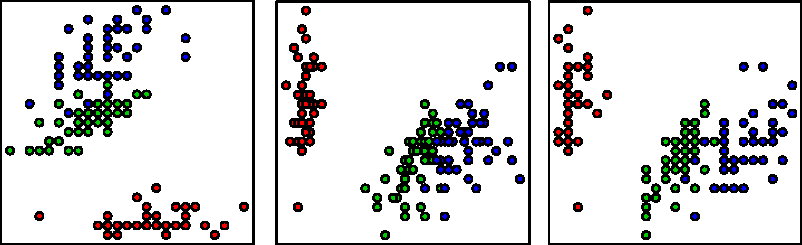
\includegraphics[height=3cm]{img/scatterplot.pdf}
\end{frame}

\begin{frame}{Data Profiling}
	\begin{block}{Data Profiling}
		"Data profiling refers to the activity of collecting data about data, i.e., metadata."\footnote{\fullcite{abedjan2018}}
	\end{block}

	\textbf{Derives metadata such as:}
	\begin{itemize}
		\item Data types and value patterns such as most frequent values.
		\item Completeness and uniqueness of columns.
		\item Number of null values and distinct values in a column.
		\item Keys and foreign keys.
		\item Occasionally functional dependencies and association rules.
		\item Discovery of inclusion dependencies and conditional functional dependencies.
	\end{itemize}
\end{frame}
